% Study of knowledge on the topic:
    % most relevant sources or prior works;
    % critical and in-depth evaluation
    % contextualize and justify the relevance of your work
    
% Usual structure:
    % Brief introduction
    % Sections related to the specific objectives;
    % Summary highlighting emerging questions on the topic;

\chapter{Literature Review} \label{chap:litreview}

This chapter reviews the research relevant to this dissertation and identifies the gaps that motivate it. Section~\ref{sec:llm-agents} follows the evolution of language models, from early statistical approaches through the Transformer architecture. Section~\ref{sec:single-agent} presents inference-time techniques, covering few-shot prompting, Chain-of-Thought, and Self-Refine. Section~\ref{sec:mas} introduces multi-agent systems, and Section~\ref{sec:interaction} organises their interaction scenarios into cooperative, adversarial, and mixed. Section~\ref{sec:negotiation} presents the NegotiationArena framework and the prior research on team-based negotiation. Finally, Section~\ref{sec:litreview-summary} draws these threads together and sets out the gaps this dissertation addresses.

\section{Language Models} \label{sec:llm-agents}

The origins of language modelling date back to the work of \textcite{6773024}, who modelled natural language as a stochastic process. Building on statistical language models, \textcite{bengio_neural_2003} proposed one of the first \acp{NLM}, predicting the next word from a fixed-length context. Subsequent work adopted \acp{RNN} and their variants, particularly \ac{LSTM}, for sequence modelling tasks such as machine translation \parencite{sutskever2014sequencesequencelearningneural}.

The introduction of the Transformer architecture \parencite{vaswani2023attentionneed} addressed some limitations of \acp{LSTM}, allowing parallelisation during training and capturing long-range dependencies through the self-attention mechanism. Applying this architecture, \textcite{Radford2018ImprovingLU} pre-trained a language model on the next-word prediction task and showed that, when followed by task-specific fine-tuning, it achieved state-of-the-art performance on common-sense reasoning, question answering, and many other tasks. GPT-2 \parencite{Radford2019LanguageMA} demonstrated that sufficiently large language models can perform downstream tasks such as summarisation, translation, and question answering without task-specific fine-tuning.

The increase in the number of parameters, dataset size, and training compute of language models continued, supported by the power-law relationship identified by \textcite{kaplan2020scalinglawsneurallanguage}, which showed that an increase in these three components led to an improvement in performance. As models grew, so did the computational costs and risks associated with their deployment. Models also differ in how they are distributed. Some are only accessible through an API, while others are released as open-weight and made publicly available (e.g., LLaMA \cite{grattafiori2024llama3herdmodels}, Mistral \cite{jiang2023mistral7b}, DeepSeek \cite{deepseekai2025deepseekv32pushingfrontieropen}). Table \ref{tab:llm-parameters} compares some of the main families of models.

Large language models have high memory requirements, often more than a single GPU can hold. Post-training quantization reduces this footprint by storing the weights at a lower numerical precision. \textcite{dettmers2022llmint88bitmatrixmultiplication} propose LLM.int8(), an 8-bit quantization method that halves the memory required for inference without measurable loss in quality, released as the open-source \texttt{bitsandbytes}\footnote{\url{https://github.com/bitsandbytes-foundation/bitsandbytes}} library. We use it to quantise several open-weight models so that they fit within the hardware available for our experiments.

\begin{table}
\centering
\small
\caption{Comparison of different models. For \ac{MoE} models, parameters are denoted as \textit{Total / Active}.}
\label{tab:llm-parameters}
\begin{tabular}{llll}
\toprule
\textbf{Model} & \textbf{Parameters} & \textbf{Licence} & \textbf{Notes} \\
\midrule
\multicolumn{4}{l}{\textit{OpenAI}} \\
GPT-1 & 117M & Open-weights & \cite{Radford2018ImprovingLU, Radford2019LanguageMA} \\
GPT-2 & 117M--1542M (4 variants) & Open-weights & \cite{Radford2019LanguageMA} \\
GPT-3 & 125M--175B (8 variants) & Proprietary & \cite{NEURIPS2020_1457c0d6} \\
GPT-4, GPT-5 & Undisclosed & Proprietary & \cite{openai2024gpt4technicalreport, singh2025openaigpt5card} \\
GPT-OSS & 117B/5.1B, 21B/3.6B & Open-weights & MoE \cite{openai2025gptoss120bgptoss20bmodel} \\
\midrule
\multicolumn{4}{l}{\textit{Google}} \\
Gemini 1.0--3 & Undisclosed & Proprietary & \cite{geminiteam2025geminifamilyhighlycapable, comanici2025gemini25pushingfrontier, google2025gemini3} \\
Gemma & 2B, 7B & Open-weights & \cite{gemmateam2024gemmaopenmodelsbased} \\
Gemma 2 & 2B, 9B, 27B & Open-weights & \cite{gemmateam2024gemma2improvingopen} \\
Gemma 3 & 1B, 4B, 12B, 27B & Open-weights & Multimodal \cite{gemmateam2025gemma3technicalreport} \\
\midrule
\multicolumn{4}{l}{\textit{Meta}} \\
LLaMA 1 & 7B, 13B, 33B, 65B & Open-weights & \cite{touvron2023llamaopenefficientfoundation} \\
LLaMA 2 & 7B, 13B, 70B & Open-weights & \cite{touvron2023llama2openfoundation} \\
LLaMA 3 & 8B, 70B, 405B & Open-weights & \cite{grattafiori2024llama3herdmodels} \\
LLaMA 4 & 109B/17B, 400B/17B & Open-weights & MoE \cite{meta2025llama4} \\
\midrule
\multicolumn{4}{l}{\textit{Anthropic}} \\
Claude 3, 4.5 & Undisclosed & Proprietary & \cite{TheC3, anthropic2025claudesonnet45systemcard, anthropic2025claudeopus45systemcard} \\
\midrule
\multicolumn{4}{l}{\textit{DeepSeek}} \\
DeepSeek-R1 & 671B/37B & Open-weights & MoE \cite{Guo_2025} \\
\bottomrule
\end{tabular}
\end{table}

\section{Inference-Time Techniques} \label{sec:single-agent}

Beyond simple improvements in performance, scaling also brought new capabilities that could not be predicted by extrapolating the performance of smaller models. \textcite{wei2022emergentabilitieslargelanguage} refers to them as \textit{emergent abilities}, including the ability to learn from examples (Few-Shot prompting, \cite{NEURIPS2020_1457c0d6}) and to think step-by-step (Chain-of-Thought, \cite{wei_chain--thought_2023}). 

Applied at inference time through prompting alone, without any weight updates, these techniques avoid the computational cost inherent in fine-tuning, which grows with the model's parameter count. These techniques have been widely adopted for their strong results, and the following subsections detail the ones most relevant to this work.

\subsection{Few-Shot Prompting} \label{sec:few-shot}

\textcite{NEURIPS2020_1457c0d6} showed that a sufficiently large language model can learn a new task from a few input-output examples placed in its prompt, with no gradient updates. They called this \textit{in-context learning} and identified three regimes by the number of demonstrations provided: \textit{zero-shot}, only a natural language description of the task; \textit{one-shot}, a description of the task and a single example; and \textit{few-shot}, a description of the task and several examples (Table~\ref{tab:few-shot}). In the few-shot setting, GPT-3 sometimes matched or surpassed the state-of-the-art fine-tuned models \parencite{NEURIPS2020_1457c0d6}. 

\begin{table}
\centering
\small
\caption{The same task posed in the zero-, one-, and few-shot regimes. In each case, the model receives the demonstrations followed by an incomplete query (\texttt{cheese =>}) and is expected to produce the completion; only the number of demonstrations changes. Adapted from \textcite{NEURIPS2020_1457c0d6}.}
\label{tab:few-shot}
\begin{tabular}{@{}lp{0.6\linewidth}@{}}
\toprule
\textbf{Regime} & \textbf{Prompt} \\
\midrule
Zero-shot & \ttfamily Translate English to French: \newline cheese => \\
\midrule
One-shot & \ttfamily Translate English to French: \newline sea otter => loutre de mer \newline cheese => \\
\midrule
Few-shot & \ttfamily Translate English to French: \newline sea otter => loutre de mer \newline plush giraffe => girafe peluche \newline cheese => \\
\bottomrule
\end{tabular}
\end{table}

\subsection{Chain-of-Thought} \label{sec:cot}

Depending on how Chain-of-Thought is implemented, it can be classified as Zero-Shot-CoT \parencite{kojima2023largelanguagemodelszeroshot} if we simply attach an instruction that elicits reasoning (e.g., ``Let's think step by step'') or Few-Shot-CoT \parencite{wei_chain--thought_2023} if we also accompany it with examples of reasoning traces. 

This technique not only improves the interpretability of models, as the reasoning traces provide a window into the decision process, but also improves the reasoning performance because dividing a complex problem into sub-problems reduces the risk of overlooking details \parencite{zhang2023ignitinglanguageintelligencehitchhikers}.

The NegotiationArena framework \parencite{bianchi_how_2024}, adopted in this work, relies on Zero-Shot-CoT. In every game, each move an agent makes is accompanied by a private \texttt{<reason>} block in which the model is asked to reason step by step before committing to an action (Listing~\ref{lst:reason-snippet}).

\begin{lstlisting}[float=htbp,caption={The \texttt{<reason>} instruction from the Buy-Sell prompt.},label={lst:reason-snippet}]
You can reason step by step on why you are A) proposing, B) rejecting
and C) accepting a trade with:

<reason> [add reasoning] </reason>  add as much text as you want

This information will not be sent to the other player. It is just for
you to keep track of your reasoning.
\end{lstlisting}

\acp{LRM} that internalise \ac{CoT} through reinforcement learning \parencite{openai2024openaio1card, Guo_2025} have become state-of-the-art, achieving a significant leap in performance, especially in coding and mathematical capabilities. \textcite{Shojaee_Mirzadeh_Alizadeh_Horton_Bengio_Farajtabar_2025} analysed the advantages of \acp{LRM} and identified three different performance regimes. For low-complexity problems, standard models often surpass \acp{LRM} while being more token-efficient. For medium-complexity problems, \acp{LRM} demonstrate a leap in performance, with their reasoning effort increasing alongside problem complexity. Nevertheless, beyond a certain complexity threshold, \acp{LRM} collapse, and both model types demonstrate a complete incapacity to solve the problem.

\subsection{Self-Refine} \label{sec:self-refinement}

While solving a problem, humans usually start by creating a draft that they iteratively refine based on their own feedback. This is the inspiration for the Self-Refine technique proposed by \textcite{madaan_self-refine_2023}, which breaks down the generation process into three steps: (1) the model generates an initial draft, (2) generates feedback, and (3) based on this feedback, refines the answer (Figure~\ref{fig:self-refine}). 

\begin{figure}
    \centering
    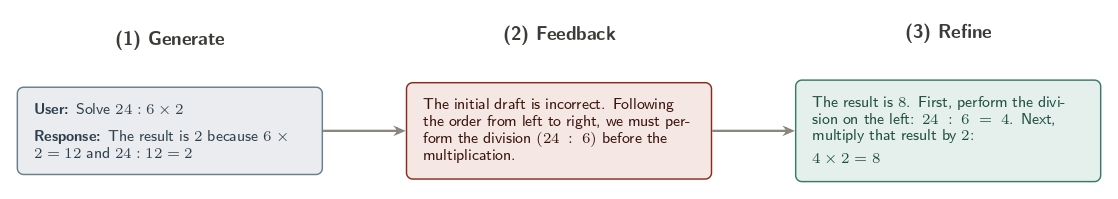
\includegraphics[width=1\linewidth]{figures/literature_review/self_refine_example.jpg}
    \caption{Example of the Self-Refine process. The model generates feedback on its initial output and uses it to produce an improved final response.}
    \label{fig:self-refine}
\end{figure}

Self-Refine is one instance of \textit{self-correction}, which \textcite{kamoi-etal-2024-llms} define as refining responses from \ac{LLM}s using \ac{LLM}s at inference time, possibly with external tools or knowledge. They distinguish \textit{intrinsic} self-correction, in which the model generates its own feedback, from self-correction that draws on external feedback, such as code interpreters, retrieved knowledge, or fine-tuned critics.

The evidence for intrinsic self-correction is mixed. \textcite{kamoi-etal-2024-llms} find that, on general tasks, no prior work shows reliable evidence of successful self-correction through in-context learning alone; the reported gains come instead from external feedback, such as executing generated code, or from large-scale fine-tuning.

This dissertation applies self-correction in both senses. Self-Refine (Section~\ref{sec:self-refine}) is intrinsic since its feedback is generated by the model itself without access to external information. The parse-error retry loop (Section~\ref{sec:retry-ablation}) is externally grounded, since during the feedback phase the agent receives the parser's error as external feedback.

\section{Multi-Agent Systems}\label{sec:mas}

From the Manhattan Project to the Space Programme, most major accomplishments in history came not from individuals alone, but from the cooperation and competition of many. The same intuition motivates the study of Multi-Agent Systems (MAS), defined by \textcite{wooldridge2002introduction} as systems of several agents that interact with one another, typically by exchanging messages.

Multi-Agent Systems existed long before \acp{LLM} became popular (Figure \ref{fig:mas_evolution}), dating back to the 1970s with distributed problem solving. In recent decades, deep reinforcement learning and \acp{LLM} have significantly expanded \acs{MAS} capabilities \parencite{ORBi-3d2db975-4cd3-46c6-84c3-a0b578b16b12}.

\begin{figure}
    \centering
    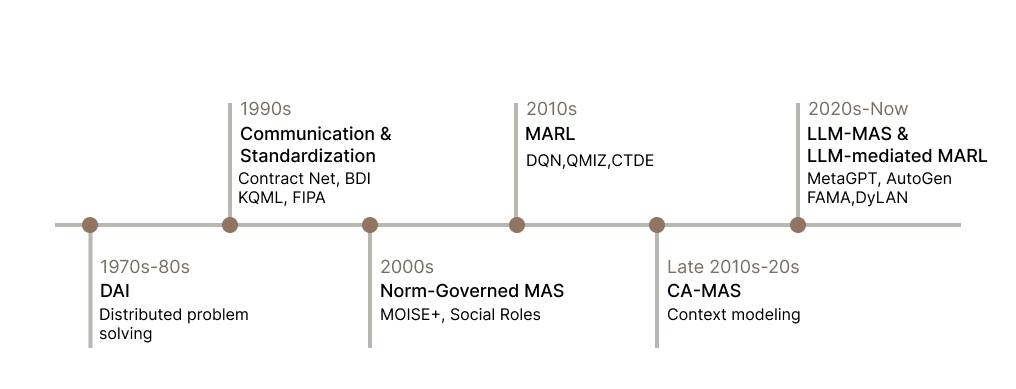
\includegraphics[width=1\linewidth]{figures/MAS_evolution.png}
    \caption{Evolution of MAS paradigms. Adapted from \textcite{ORBi-3d2db975-4cd3-46c6-84c3-a0b578b16b12}.}
    \label{fig:mas_evolution}
\end{figure}

%Following \textcite{wooldridge2002introduction}, an agent is a computer system capable of independent action on behalf of its user or owner, able to figure out for itself what it needs to do to satisfy its design objectives rather than being told explicitly at every step. A \ac{MAS} is a system of several agents that interact with one another, typically by exchanging messages.

%TODO: Agent Definition
%TODO: LLM-Based Agent Definition

\textcite{Li2024} proposed a unified framework for \ac{LLM}-based \acs{MAS}, identifying the following five components:

\begin{itemize}
    \item Profile: An agent’s identity and characteristics (roles, goals, and personalised traits).
    \item Perception: An agent’s perception of the environment to acquire knowledge and experience.
    \item Self-Action: An agent’s ability to make decisions and execute actions based on its perception and internal state.
    \item Mutual Interaction: Communication and collaborative coordination among agents.
    \item Evolution: An agent’s reflection on its actions and behaviours to progressively improve its intelligence and experience.
\end{itemize}

\section{Interaction Scenarios}\label{sec:interaction}
According to \textcite{Li2024}, interaction scenarios in LLM-based Multi-Agent systems can be classified as cooperative, adversarial, or mixed. 

\subsection{Cooperative}

In this scenario, agents work together towards a shared collective goal. It usually follows these steps: after setting a common goal, agents decompose the task and use communication and negotiation to reach a consensus \parencite{tran2025multiagentcollaborationmechanismssurvey}. 

Inspired by human group dynamics, \textcite{chen2023agentversefacilitatingmultiagentcollaboration} propose AgentVerse, a framework for problem-solving. Its process is divided into four steps. First, a recruiter agent determines the group's composition by writing a set of expert descriptions, one per agent, based on the goal. Then, the selected agents collaborate to decide on the actions to take. Finally, the chosen action is executed, transitioning the environment to a new state, which is then evaluated. In this last stage, a feedback mechanism assesses the difference between the new state and the desired goal and returns verbal feedback that describes where the current solution falls short and suggests how to improve it. This evaluator can be a human, in a human-in-the-loop setting, or another agent that produces the feedback automatically, depending on the implementation. If the goal is not yet met, the feedback is routed back to the recruitment stage, which uses it, together with the goal, to adjust the group's composition in the next round. This cycle repeats until the goal is reached.

\textcite{3692070.3692537} introduce collaborative debate as a way to improve the factual validity and the mathematical and strategic reasoning across a number of tasks. First, a set of LLMs generates possible answers to a question. Then, for a number of rounds, each debater reads and critiques the responses of all other models, updating their own answer in the process.

\textcite{chen2024reconcileroundtableconferenceimproves} propose RECONCILE, a round-table conference in which diverse \acp{LLM} collaborate to solve reasoning problems. Each agent first generates an answer, a \ac{CoT} explanation, and a confidence estimate. Then, over several rounds, every agent reads the grouped answers, explanations, and confidences of the others and revises its own response, attempting to convince the rest. At the end of each round, a confidence-weighted vote chooses the team answer, and the discussion stops once the agents reach a consensus or a maximum number of rounds is exceeded. 

\subsection{Adversarial}
Competition occurs when agents have conflicting objectives and seek to maximise their own interests, often with limited resources \parencite{tran2025multiagentcollaborationmechanismssurvey}.

Inspired by \textcite{irving2018aisafetydebate}'s idea of debate as an approach to \ac{AI} alignment, \textcite{khan_debating_2024} implement an information-asymmetric debate where two expert models (debaters) argue for different sides over N rounds, attempting to persuade a weaker model (judge) that must identify the correct side. This work has the objective of answering the question ``can weaker models assess the correctness of stronger models?'', motivated by a future where humans need to supervise more powerful models.

% Another example of debate is the ChatEval framework by \textcite{chan2023chatevalbetterllmbasedevaluators}, designed to evaluate the quality of responses generated by different models. At the end of the debate, instead of asking the debater agents to reach a consensus, the framework aggregates the individual judgements: by majority vote when the task is a direct comparison, or by averaging the individual scores when a numerical score is required.

\subsection{Mixed}

Some scenarios combine features of both cooperative and adversarial interactions. This is the case in \textit{Diplomacy} \parencite{doi:10.1126/science.ade9097}, where seven players negotiate over a map of Europe with the aim of controlling as many supply centres as possible. In this game, players collaborate with some by forming alliances and compete with others to gain territory.

\section{Negotiation} \label{sec:negotiation}

%Multiple works evaluate \acp{LLM}' strategic reasoning on game-theoretic scenarios. \textcite{feng2025surveylargelanguagemodelbased} distinguish two types of games: choice-focused, if there is little to no communication between the participants (e.g., Poker \cite{zhuang2025pokerbenchtraininglargelanguage}), or communication-focused, when communication is the main component of the game (e.g., Negotiation \cite{bianchi_how_2024}). The latter category, and negotiation in particular, is the focus of this dissertation and is examined in detail in Section~\ref{sec:llm-negotiators}.

\textcite{Jennings2001AutomatedNegotiation} describe negotiation as the process by which a group of agents reach a mutually acceptable agreement on some matter.

\subsection{LLMs as Negotiators} \label{sec:llm-negotiators}

Negotiation is a particularly interesting evaluation scenario for \acp{LLM} since, in order to be successful at it, agents need to interpret the competitor's actions and underlying intentions so that they can adapt their strategy accordingly. \textcite{bianchi_how_2024} proposed NegotiationArena, an open-source framework for evaluating and probing the negotiation abilities of \ac{LLM} agents. We adopt this framework throughout the dissertation, studying how open-weight models negotiate within it.

The framework implements three scenarios, which we describe in full in Section~\ref{sec:games}: 
\begin{itemize}
    \item \textbf{Multi-Turn Ultimatum Game:} a multi-round extension of the classical Ultimatum Game in which one agent proposes how to split a pot and the other accepts, counters or rejects.

    \item \textbf{Trading Game:} each agent holds a set of resources and exchanges proposals with the goal of maximising its own holdings.

    \item \textbf{BuySell Game:} an incomplete-information game in which a seller and a buyer, each with a private valuation, negotiate the price of an item.
\end{itemize}

%Esta parte foi comentada, porque estava a repetir em detalhe os jogos aqui e na metodologia
%\begin{itemize}
%    \item \textbf{Multi-Turn Ultimatum Game:} The Ultimatum Game is a classical game in game theory where one agent starts with all of the game resources and, in order to keep part of them, the agent must propose a split and convince another agent to accept it. If the agent rejects it, the game is over and they both get nothing. \textcite{bianchi_how_2024} made a modification in relation to the classical game, allowing multiple turns, so there could be negotiation between the agents. The agent who secures more resources is considered the winner.
%    \item \textbf{Trading Game}: In this game, each agent has a set of resources and a goal (e.g., maximise its total resources). For a number of rounds, the agents make proposals to each other until one accepts a proposal. Similar to the Ultimatum Game, the agent who obtains more resources is considered the winner.
%    \item \textbf{BuySell}: This scenario involves two agents with opposing roles: a \textit{seller}, who owns an item and wants to sell it at the highest possible price, and a \textit{buyer}, who wants to acquire it at the lowest. The two must negotiate until they agree on a price or one of them walks away. This is an incomplete information game since each agent has private information (the seller's cost and the buyer's willingness to pay), which is not directly observable by the other party. An agent wins if the agreed price is closer to the opponent's valuation than to its own.
%\end{itemize}

The framework uses two metrics: win rate and average payoff. By analysing them, we can obtain meaningful comparisons of the models' ability to negotiate with others.

Beyond comparing models against each other, \textcite{bianchi_how_2024} also probe how social behaviour shapes negotiation outcomes, analysing the impact of two personas: a \textit{cunning} agent, instructed to be sly and to insult and humiliate its opponent, and a \textit{desperate} agent, instructed to feign desperation and beg for a better deal.  

In every game, both personas raised win rate, and, in most cases, average payoff over the no-persona baseline. The effect is more pronounced in the Ultimatum Game, where a default second player almost never secures more than half the pot, yet a desperate or cunning persona enables it to win far more often. The cunning persona is nonetheless high-risk: in the Ultimatum Game it lifts the win rate to 82\% while leaving the average payoff close to the baseline, because its aggressive tactics often end in no agreement and a zero payoff for both sides. This dissertation replicates these social-persona experiments on open-weight models in Section~\ref{sec:personas}, using the same two personas.

\subsection{Team-Based Negotiation}

Most negotiation research, whether classical or \ac{LLM}-based, models each party as a single agent. Yet many real negotiations (for example, two countries negotiating a trade agreement) are conducted by a \textit{negotiation team}. \textcite{S_nchez_Anguix_2013} define a negotiation team as a group of interdependent people who join and act together as a single negotiation party because of their shared interests in a negotiation. Their study predates \ac{LLM}s and uses an agent-based setting where every member has an explicit utility function and concedes over time according to a fixed tactic. In it, they propose four \textit{intra-team strategies} that determine \textit{what} decisions the team takes, and \textit{how} and \textit{when} it takes them:

\begin{itemize}
    \item \textbf{Representative (RE):} a single member negotiates on behalf of the team, which reduces the team to an ordinary bilateral negotiation and guarantees no unanimity.  
    \item \textbf{Similarity Simple Voting (SSV):} a mediator gathers one proposal per member and forwards the offer with the most votes (plurality), accepting the opponent's offer by majority.
    \item \textbf{Similarity Borda Voting (SBV):} similarly to SSV, a mediator gathers one proposal per member, but members \textit{rank} the proposed offers and a Borda count selects the one to send, while acceptance requires unanimity.
    \item \textbf{Full Unanimity Mediated (FUM):} a more active mediator builds the offer one issue at a time, after a pre-negotiation phase in which members hand over the issues they do not care about, so that every decision is unanimous.
\end{itemize}

In parallel, as seen in Section~\ref{sec:interaction}, several works show that letting several \ac{LLM}s deliberate before answering can improve the quality of their output \parencite{chen2024reconcileroundtableconferenceimproves, 3692070.3692537}. 

Bringing these two lines together, this dissertation replaces one negotiation party with a team of \acp{LLM} that independently draft a move, discuss it over several rounds as in RECONCILE \parencite{chen2024reconcileroundtableconferenceimproves}, and settle on a single move with a Borda count. We take the Borda count from the Similarity Borda Voting strategy of \textcite{S_nchez_Anguix_2013}, but unlike SBV, acceptance is not a separate unanimity decision but simply one more candidate on the ranked slate. To test whether model diversity helps, as RECONCILE suggests, we also compare homogeneous teams against heterogeneous teams. Section~\ref{sec:team-negotiation} details this design.

\section{Summary}\label{sec:litreview-summary}

This chapter reviewed the work this dissertation builds on, from language models to multi-agent negotiation.

The opening section followed the evolution of language models, from early statistical approaches through the Transformer architecture and the GPT family, open-weight releases and post-training quantization.

Section~\ref{sec:single-agent} turned to inference-time techniques covering few-shot prompting and Chain-of-Thought, which the NegotiationArena framework adopts through its per-move \texttt{<reason>} block, and Self-Refine, a draft, feedback and rewrite loop. 

Section~\ref{sec:mas} introduced multi-agent systems and Section~\ref{sec:interaction} organised their interaction scenarios as cooperative, adversarial, or mixed. Two cooperative approaches are particularly relevant to this work: collaborative debate \parencite{3692070.3692537} and the RECONCILE round-table \parencite{chen2024reconcileroundtableconferenceimproves}, both of which report better answers when several models deliberate before responding.

The closing section focused on negotiation. It presented NegotiationArena \parencite{bianchi_how_2024}, the framework adopted throughout this dissertation. On team-based negotiation, \textcite{S_nchez_Anguix_2013} studied negotiation teams before \acp{LLM}. This dissertation takes the Borda-count voting from their Similarity Borda Voting strategy and combines it with the deliberation idea from RECONCILE \parencite{chen2024reconcileroundtableconferenceimproves} to replace a single party with a team of models.

Taken together, these threads expose the gaps this dissertation addresses. NegotiationArena was evaluated only on proprietary models, some of which have since been deprecated, leaving open how the smaller, openly available models negotiate in the same scenarios and whether the social-persona impact reported for GPT-4 carries over to them. Self-Refine has not been tried in negotiation. Although negotiation teams were studied before \acp{LLM}, and \ac{LLM} deliberation has improved reasoning elsewhere, the two have not been combined. This dissertation addresses these gaps by benchmarking nine open-weight models across three families and tiers on three games, replicating the NegotiationArena social-persona experiments, and studying Self-Refine and a deliberating team of models as inference-time interventions. In doing so, it lays the groundwork for the methodology in Chapter~\ref{chap:methodology} and the results in Chapter~\ref{chap:results}.